%課題研究レジュメテンプレート ver. 1.2

\documentclass[uplatex]{jsarticle}
\usepackage[top=20mm,bottom=20mm,left=20mm,right=20mm]{geometry}
\usepackage[T1]{fontenc}
\usepackage{txfonts}
\usepackage{wrapfig}
\usepackage[expert,deluxe]{otf}
\usepackage[dvipdfmx,hiresbb]{graphicx}
\usepackage[dvipdfmx]{hyperref}
\usepackage{pxjahyper}
\usepackage{secdot}

\makeatletter
  \renewcommand{\section}{%
    \if@slide\clearpage\fi
    \@startsection{section}{1}{\z@}%
    {\Cvs \@plus.5\Cdp \@minus.2\Cdp}% 前アキ
    {.5\Cvs \@plus.3\Cdp}% 後アキ
    %{\normalfont\Large\headfont\raggedright}}
    {\normalfont\raggedright}}

  \renewcommand{\subsection}{\@startsection{subsection}{2}{\z@}%
    {\Cvs \@plus.5\Cdp \@minus.2\Cdp}% 前アキ
    {.5\Cvs \@plus.3\Cdp}% 後アキ
    %{\normalfont\large\headfont}}
    {\normalfont}}

  \renewcommand{\subsubsection}{\@startsection{subsubsection}{3}{\z@}%
    {\Cvs \@plus.5\Cdp \@minus.2\Cdp}%
    {\z@}%
    %{\normalfont\normalsize\headfont}}
    {\normalfont}}
\makeatother
%ここから上を編集する必要はない.




\title{\vspace{-14mm}大学祭来場者数を予測する数理モデル}
\author{PMコース 矢吹研究室 1342045 川手 元稀}
\date{}%日付を入れる必要はない.
\pagestyle{empty}%ページ番号は振らない.
\begin{document}
\maketitle




\section{研究の背景}

この研究に着手した背景が2つある.

1点目に津田沼祭の来場者数は増加傾向にあることである.2015年度の来場者数は過去最大の2万人超えになった.しかし,来場者数が増加することで事故,傷害といったリスクが高まる.
例えば,人が多すぎてステージ前で将棋倒しになり負傷者を出したことや,人通りが多く子どもが迷子になることなど様々である.私は事前に来場者数の予測ができたらと考えた.

2点目に大学祭実行委員の活動時間の長さである.受付,警備は9時間もの間行なっている.実行委員の活動は本祭時間外でも行われる.例えば企画のリハーサル,夜間警備,校内清掃等を行っている.このように過酷な活動が原因で体調不良者が出てしまう傾向にある.私は警備・受付の時間を軽減できれば良いと考えた.


%\begin{wrapfigure}[行数]{r}{幅}%行数はオプションだが,調整しないとうまくいかない.
\begin{wrapfigure}[8]{r}{8cm}
\vspace*{-\intextsep}
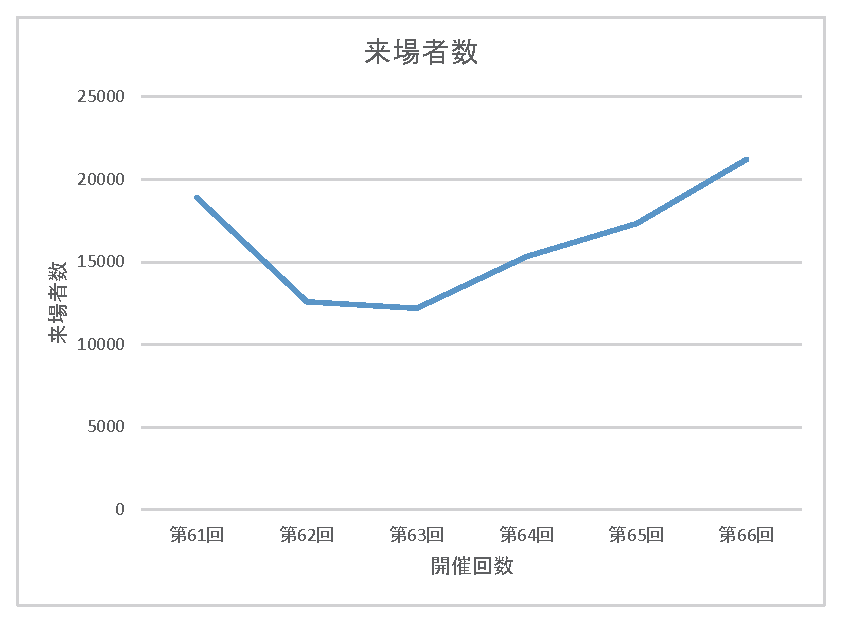
\includegraphics[width=8cm,clip]{visitors.pdf}
\caption{津田沼祭来場者数}\label{図1}
\end{wrapfigure}


\section{研究の目的}
本研究は2段階に分かれる.

\begin{enumerate}
\item 来場者数を事前に予測して過去に同じような来場者数が出ている年を参考に事故のリスクを予測・対応ができるようになること.
\item 本祭中の警備や受付に掛ける時間を少しでも軽減し,来場者数に応じて実行委員を適正人数で運営できることができること.
\end{enumerate}

\section{プロジェクトマネジメントとの関連}

プロジェクトマネジメントとの関連については以下に記載する.

\begin{enumerate}
\item 人的資源マネジメントの分野で関連がある.来場者数に応じて警備や受付を適正人数で行えるからである.実行委員の仕事を軽減することが可能になり,個人のモチベーションの向上に繋がるからだ.
\item リスクマネジメントの分野で関連がある.来場者を予測することでリスクを洗い出し対応策を過去の事例から考えられるからだ.
\item コストマネジメントの分野で関連がある.来場者数に応じて実行委員の活動時間を軽減できるためである.
\end{enumerate}


\section{研究の方法}

\subsection{来場者数の計測方法}

毎年,大学祭実行委員会では門から入場した人数を来場者数としている.同じ人が入場した場合でもカウントを行っている.
\subsection{データの収集について}

過去9年分の大学祭のデータを大学祭実行委員会の許可を取り,収集を行った.データ項目は各年代の来場者数,模擬店の運営人数,開催日,開催曜日である.

天候にも関係があると考え開催日の天候のデータを収集した\cite{a}.

\subsection{データの解析方法}

データの解析方法を以下に記載する.

\begin{enumerate}
\item 開催した曜日を数量化理論Ⅰを使用し質的データを量的データに変換する.
\item 来場者数を目的変数とし,開催した曜日,3日間の降水量,ブースを運営している人数,ブースの数を説明変数として回帰分析を行い予測式を立てる.
\item 分析ツールRを利用し集めたデータ項目の中で来場者数に最も関係しているデータを調査する\cite{b}.

\end{enumerate}

\section{現在の進捗状況}

結果は過去のデータが少なかったため有効性の高い予測式は立てられなかった.

現在までで集めたデータを次に繋げるため,来場者数に関係性の高いデータをRで調査した\cite{b}.
結果は運営人数,1日目の降水量に関係性があった.

1日目の降水量に関しては本祭1日目に雨が降ると来場者数は減少する傾向にある.理由は過去9年分の天候データは初日に雨が降る確率が高かった.そのため,減少傾向にあると考える.

運営人数に関しては人数が増加すると来場者数は増加する傾向にある.理由は運営していると食材や材料等が無くなり買い出しに行った人が再度入場したためである.データを見ると1人につき約3回入場した計算になった.詳細な結果は以下に記載する.

\begin{table}[hbtp]
  \caption{本祭3日間の降水量のデータ}
  \label{table:data_type}
  \centering
  \begin{tabular}{lrrr}
    \hline
    開催回数 & 1日目の降水量(mm)  & 2日目の降水量(mm)  &  3日目の降水量(mm)  \\
    \hline \hline
    61回 & 1 & 0 & 0 \\
    62回 & 6 & 0 & 0 \\
    63回 & 7 & 0.5 & 0 \\
 64回 & 0 & 0 & 0 \\
 65回 & 0 & 0 & 0 \\
 66回 & 0 & 0 & 0 \\
    \hline
  \end{tabular}
\end{table}

\begin{wraptable}[4]{r}{4cm}
\vspace*{-\intextsep}
\caption{来場者数との関係性}
\begin{tabular}{lr}
\hline
運営人数 & 2.895 \\
1日目降水量& -724.074  \\
\hline
 \end{tabular}
\end{wraptable}


\section{今後の計画}

以下のように研究を進める計画である.

\begin{enumerate}
\item 学校が計測しているデータを集め,予測式の有効性を向上させる.
\item 来場者数の予測が可能になったら過去に類似している来場者数の年を見つけ出す.その年に起こった事件・事故を把握し対応を可能にする.
\end{enumerate}
\bibliographystyle{junsrt}
\bibliography{biblio}%「biblio.bib」というファイルが必要.

\end{document}